\chapter{مقدمه}\label{chap:1}

%%%%%%%%%%%%%%%%%%%%%%%%%%%%%%%%%%%%%%
%            1.0
%%%%%%%%%%%%%%%%%%%%%%%%%%%%%%%%%%%%%%
البته چالش اصلی این مسئله تنوع تصاویر طبیعی است. این تنوع حاصل تفاوت در حالت
\LTRfootnote{Pose}
است. می توانید به شکل
\ref{fig:1:variation}
ارجاع دهید.

\begin{figure}
	\centering
	\subfigure[]{\label{fig:1:variation:obj}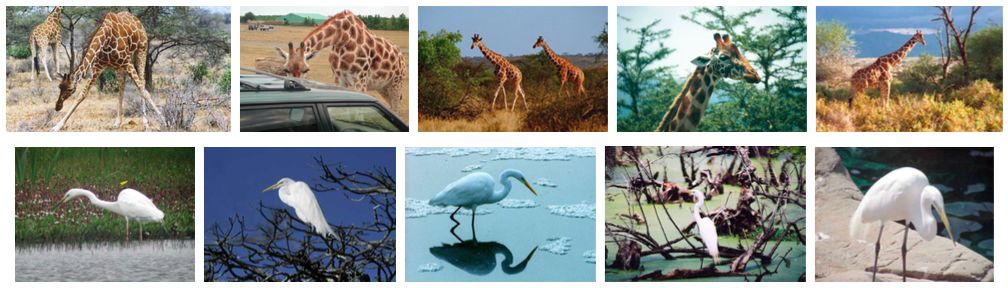
\includegraphics[width=0.9\textwidth]{var_obj}}
	\subfigure[]{\label{fig:1:variation:scene}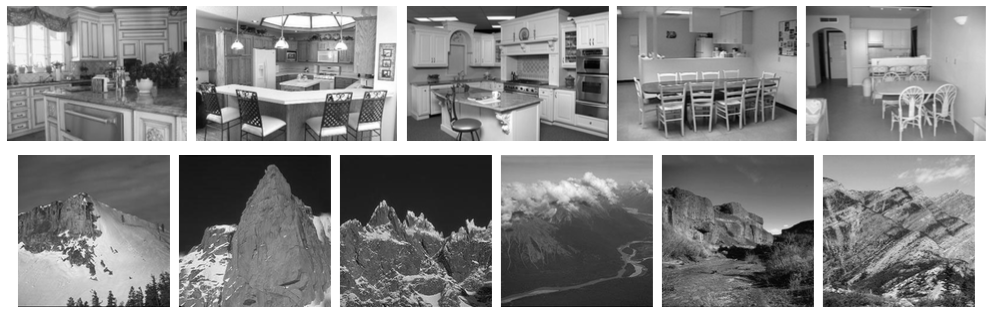
\includegraphics[width=0.9\textwidth]{var_scene}}
	\caption[نمونه‌هایی از انواع تنوع در تصاویر طبیعی که برای بازشناسی باید مورد توجه قرار بگیرد]{نمونه‌هایی از انواع تنوع در تصاویر طبیعی که برای بازشناسی باید مورد توجه قرار بگیرد\cite{phdlazeb}.
\subref{fig:1:variation:obj} اشیا معمولا به خاطر پوشیدگی و شلوغی به سختی قابل بازشناسی هستند. حیوانات از جمله اشیای غیر صلب هستند و در حالات مختلفی ظاهر می‌شوند.
\subref{fig:1:variation:scene} تصاویر صحنه‌های طبیعی مانند کوهستان دارای تفاوت درون دسته‌ای بسیار زیادی هستند. همچنین برخی تصاویر از محیط‌های داخلی (مانند آشپزخانه و اتاق نشیمن) به‌سختی از هم قابل تمایز هستند.}
	\label{fig:1:variation}
\end{figure}